\chapter{Exploratory Directions and Negative
Results}

The experimental chapters (4--7) establish a wall: on average-case
matching the advice-free baseline is near-optimal, so predictions are
robustness insurance rather than a performance lever. Before accepting
the wall as final, we pursued three directions that each \emph{tried to
get past it}: learning the predictor to squeeze out more performance
(§8.1), finding a serving regime where predictions genuinely help
(§8.2), and letting a systematic literature review point us to the
highest-value contribution (§8.3). All three returned the same answer,
and their convergence is what motivated the theorem. Each is reported
here with the evidence that closed it.

\section{Learning to rank the predictor (a negative
result)}

Chapter 5 shows that MPD consumes its predictor only through the order
it induces. This suggests a concrete way to do better: rather than
training a predictor to minimize its \emph{regression} error to the true
degrees (the standard ``predict-then-optimize'' objective), train it
with an \emph{order-aware} loss (a pairwise rank loss) so it optimizes
the quantity the algorithm actually uses. We investigated this in three
steps.

\textbf{M0: the mechanism exists} (\textbf{Figure 8.1}). With
deliberately \emph{divergent} synthetic features (one feature carrying
magnitude, another carrying order), a rank-trained linear predictor
sharply beats a regression-trained one on the decision metric: matching
ratio \(0.989\) (essentially the oracle) versus \(0.974\), while the
rank-trained predictor has \emph{worse} regression error to the truth
(MSE \(87.6\) vs \(33.4\)) but better order (Kendall-\(\tau\) \(0.058\)
vs \(0.255\)). The dissociation is real: the worse \emph{fit} gives the
better \emph{decision}. Regression is thus the wrong training objective
whenever the features separate magnitude from order, a condition M1 and
M3 below show to be rare.

\begin{figure}
\centering
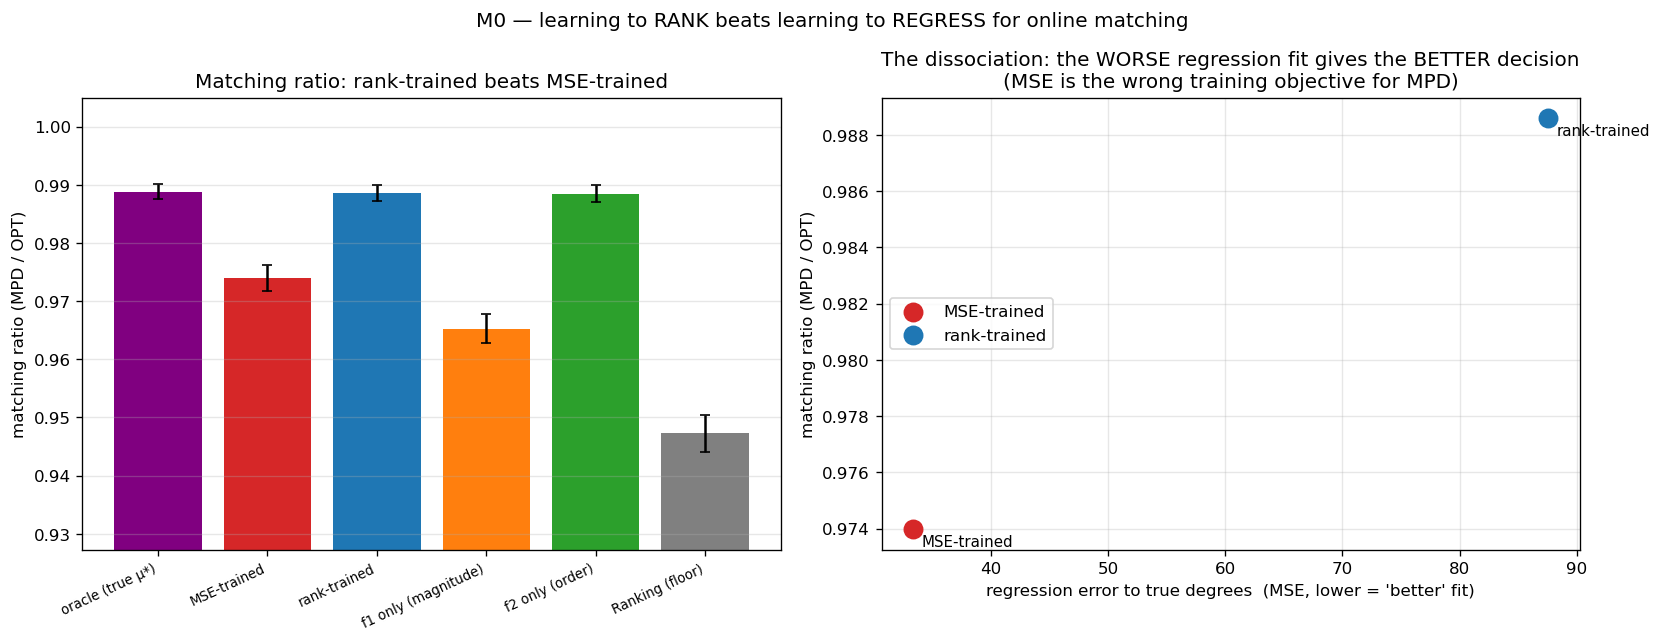
\includegraphics[width=1\linewidth,height=\textheight,keepaspectratio,alt={M0: with divergent features, rank-training beats regression on the matching ratio (left) despite a worse regression fit (right).}]{../../results/rank_vs_mse_mve.png}
\caption{M0: with divergent features, rank-training beats regression on
the matching ratio (left) despite a worse regression fit (right).}
\end{figure}

\textbf{M1: the advantage is doubly gated, and small.} Sweeping the
feature divergence and the graph difficulty, the rank-advantage is zero
when features do not induce an order/magnitude conflict, and zero on
easy instances where the baseline is already optimal (the wall, again).
It peaks at only \(+1.3\%\) of the ratio on synthetic graphs; measured
as gap-capture (§7.1) rather than as an absolute ratio, rank-training
recovers essentially the full oracle gap while regression leaves about
\(30\%\) of it unrealized, but the gap itself is small.

\textbf{M3: it disappears on real features} (\textbf{Figure 8.2}). The
decisive test uses genuine temporal features from real serving traces
(per-resource reference counts over the previous windows) to predict the
next window (150 context-length types over 500 replicas of degree 8, 40
windows, three lag features, a 60/40 train/test split). Here the rank-
and regression-trained predictors produce identical order
(Kendall-\(\tau\) \(0.126\) vs \(0.126\)) and identical matching ratio.
The order/magnitude divergence that powers rank-training arises in the
\emph{engineered} features used above. For the realistic lagged-count
features examined here, the features appear to be co-linear noisy
estimates of the same popularity, and regression recovers the order as
well as ranking does.

\begin{figure}
\centering
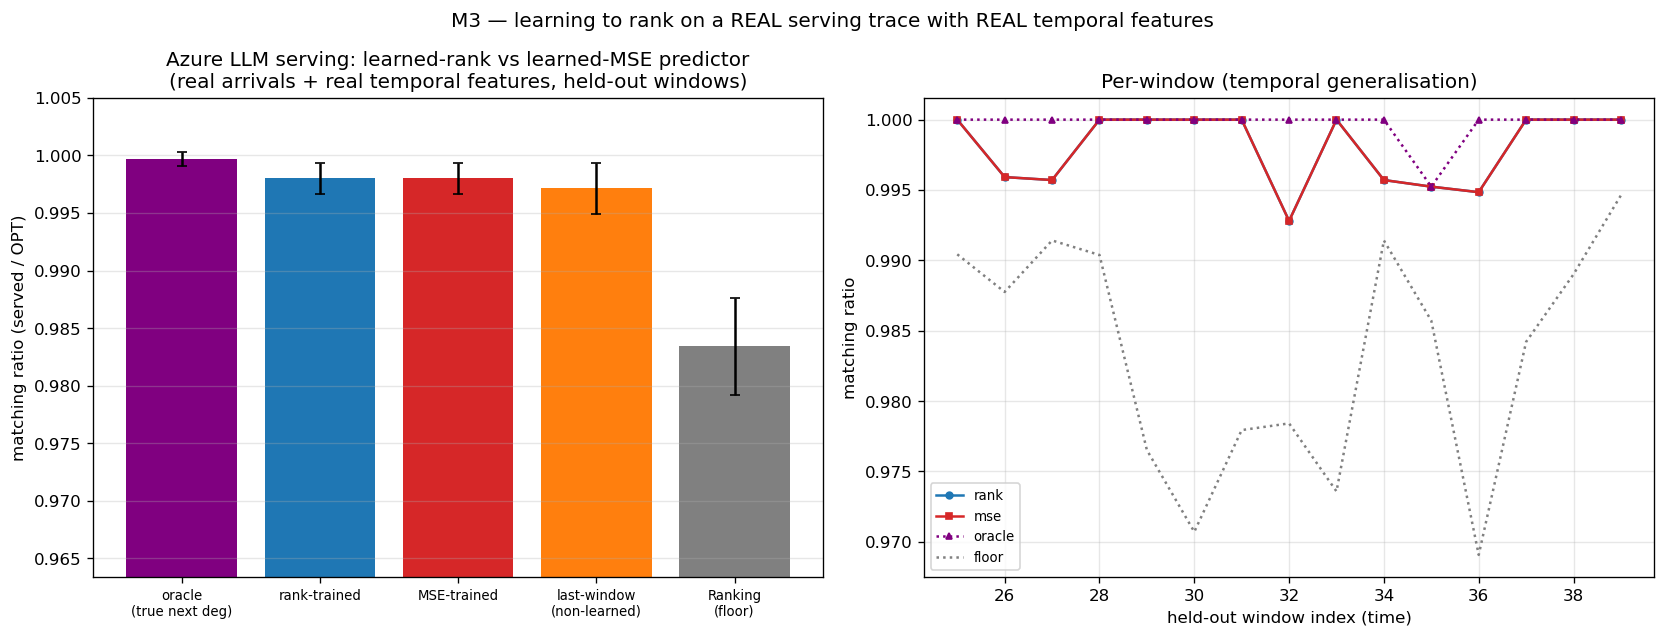
\includegraphics[width=1\linewidth,height=\textheight,keepaspectratio,alt={M3 (Azure trace, real temporal features): rank- and MSE-trained predictors are indistinguishable; the engineered divergence that powers rank-training does not arise in this experiment.}]{../../results/rank_real_trace.png}
\caption{M3 (Azure trace, real temporal features): rank- and MSE-trained
predictors are indistinguishable; the engineered divergence that powers
rank-training does not arise in this experiment.}
\end{figure}

\textbf{Verdict.} Learning the predictor with a decision-aligned loss
does not change the picture of Chapters 4--7, and we report it as a
negative result: in these experiments, the win requires a feature
divergence that did not arise on the real trace, and even where it does
the payoff is bounded by the (small) baseline-to-oracle gap. The result
is folded into the thesis as a negative that reinforces the central
finding: once a predictor is order-faithful, which a cheap historical
count already is (Chapter 7), neither a better algorithm nor a
better-trained predictor buys much on average-case matching.

\section{Rescuing the serving application with a with-predictions result
(a negative
probe)}

The serving case study (Chapter 9) recovers established systems results
and is therefore presented as a case study rather than a novelty claim.
We asked whether a new actionable with-predictions result could rescue
it. The escape, if one exists, must be a different \emph{objective}, one
on which the reactive baseline is genuinely far from optimal. The
obstacle otherwise is again the wall: every serving variant we tried
optimizes \emph{throughput} (goodput), and throughput is forgiving,
since under overload a reactive router fills capacity just as the
optimum does.

We probed the most promising candidate: an \textbf{SLO / tail objective}
(protecting a tight-SLO class of requests from being dropped) under
bursty, non-stationary load, exactly the regime where a reactive policy,
lacking foresight, might fail. Using an event-driven simulator we
compared non-predictive policies (static capacity reservation; a
reactive-adaptive policy that reserves based on \emph{observed} recent
load) against a \textbf{clairvoyant reference} that reserves based on
the \emph{actual future} burst. Two caveats belong with that design. The
reference has perfect foresight but is not a proven optimum for the SLO
objective, so it estimates what foresight is worth rather than bounding
it; and the estimate is visibly not tight, because in the moderate
regime a trivial static reservation of one slot drives tight-SLO
violations to near zero and beats the clairvoyant reference outright,
reserving for the actual future burst over-reserves there. What the
sweep does establish is one-directional and still useful: across every
regime (overload level, uniform vs bursty tight-SLO demand), the best
non-predictive policy comes within \(\le 3\%\) (\textbf{Figure 8.3}) of
a policy that knows the future exactly, so the particular thing a
forecast would supply is not what these policies are missing. Two
reasons, both robust to the sweep: protecting a tight-SLO minority needs
only a small static headroom, no forecast; and bursts are persistent
enough that reacting to observed load is almost as good as forecasting
it.

\begin{figure}
\centering
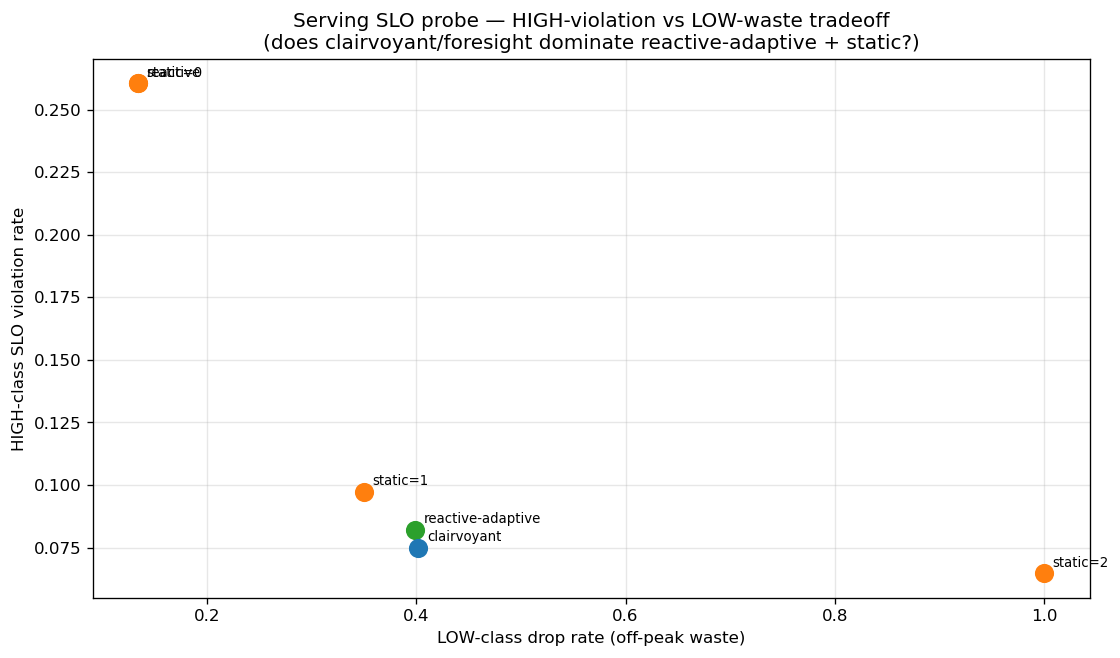
\includegraphics[width=0.6\linewidth,height=\textheight,keepaspectratio,alt={Serving SLO probe: the best non-predictive policy comes within a few percent of the clairvoyant reference, suggesting little additional value from foresight in this sweep.}]{../../results/serving_slo_probe.png}
\caption{Serving SLO probe: the best non-predictive policy comes within
a few percent of the clairvoyant reference, suggesting little additional
value from foresight in this sweep.}
\end{figure}

\textbf{Verdict.} The tail objective is also forgiving in the regimes
examined: a third face of the wall, after throughput (Chapters 4--7) and
predictor-learning (§8.1). We did not identify a benefit from foresight
within this sweep, so serving remains a case study. A regime that would
break the wall (a non-stationary or adversarial objective where the
baseline is far from optimal) is exactly the kind of setting the thesis
brackets as future work.

\section{A literature review that redirected the
work}

Deciding which of our findings were genuinely novel required a
systematic prior-art review rather than intuition: we searched from
several independent starting points and checked each candidate claim
against the primary papers rather than their abstracts. The verdicts
were sometimes deflating. The unified benchmark and the empirical study
of test-and-fallback are unoccupied and worth leading with; the
order-error finding is \emph{partially} pre-empted by ACI's Appendix D
and had to be reframed as a tightness/measure characterization rather
than a discovery (Chapter 5); and the serving results are largely
re-derivations of established systems facts, warranting their demotion
to a case study (§8.2, Chapter 9). A focused second pass confirmed that
no prior work quantifies the cost of the prefix test on strong-baseline
instances, while flagging the one risk any such result must defend
against (Choo et al.'s constructive baseline-coupling), an input to the
outlook of §10.2.

The review is itself part of the research process reported here: it
turned an undifferentiated pile of findings into a prioritized
contribution, redirected effort away from low-value elaborations toward
the theory question, and enforced the honesty guardrails carried
throughout the thesis.

\section{Synthesis: the negatives point to the same
wall}

The three explorations point the same way. A better-trained predictor
did not help on the real features tested (§8.1); a with-predictions lens
did not improve serving on the tail objective examined (§8.2); and the
literature review did not identify an established route to an easy
performance gain (§8.3). Together with the throughput results of
Chapters 4--7, these findings show that the same pattern recurs across
the objectives, algorithms and datasets examined. This recurrence
motivates the possibility that the wall reflects a structural constraint
rather than an accident, which the concluding outlook (§10.2) considers.
